\section{Elaboration Time Hardware Construction}
The methods for constructing hardware in the previous sections are all
similar in that the user directly interfaces with them. The user
directly constructs the directed subgraph of {\tt Nodes} that
implements the desired circuit and connects that subgraph to the main
graph. We refer to that class of hardware construction as 
{\it runtime} hardware construction since the hardware is
constructed as Scala is making a pass over user-written code. This
chapter discusses another class of hardware construction that we refer
to as {\it elaboration time} hardware construction since the
hardware is constructed during Chisel elaboration. This class of
hardware construction is useful since it is not always possible or
desirable for the user to construct the circuit as they are building
up the Chisel graph. The remainder of this chapter presents the
interface for writing elaboration time hardware construction routines
and three examples of how to use that interface.

\subsection{Elaboration Time Hardware Construction Interface}
The Chisel compiler mantains a list of functions that it invokes
during elaboration time to refine the input user graph of 
{\tt Nodes}. These functions must adhere to the interface described in
Figure~\ref{fig:transforms}. The bodies of the functions in
Figure~\ref{fig:transforms1} varies from transformation to
transformation but will usually follow two phase format. The first
phase performs some analysis on the Chisel graph to collect
information, e.g. find all Reg nodes. The second phase will then use
the information from the first phase to construct a circuit and
perform some transformation on the graph, e.g. generate an enable
circuit for every Reg node and connect the circuit into the Reg node.

\begin{figure}[htb]
\centering
  \begin{subfigure}[t]{0.48\textwidth}
  \centering
  \caption{Elaboration Time Functions}
  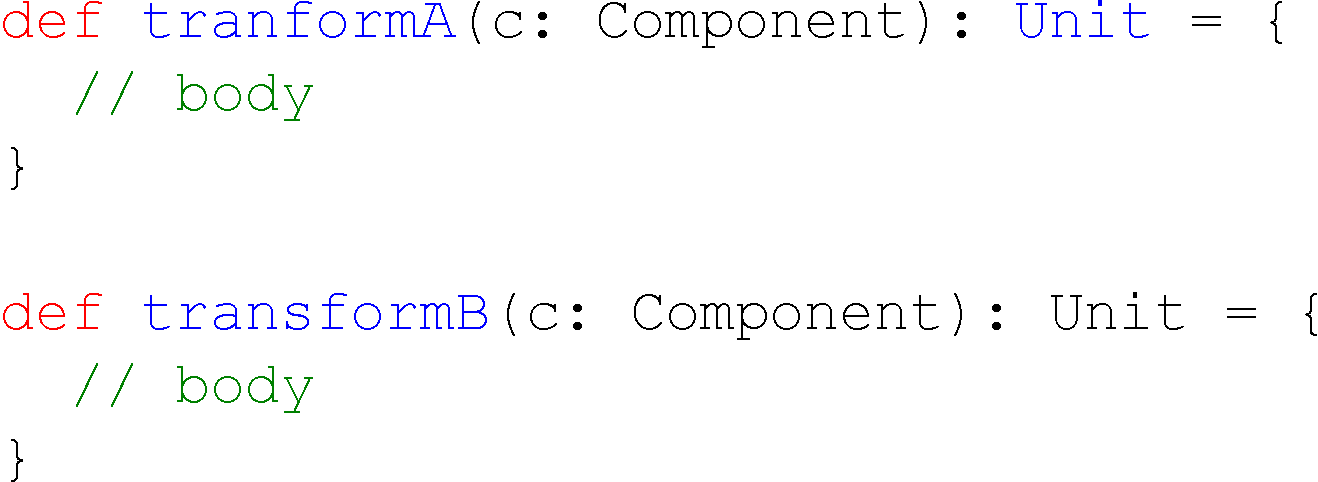
\includegraphics[width=0.9\textwidth]{figures/transform1.pdf}
  \label{fig:transform1}
  \end{subfigure}
  \hfill
  \begin{subfigure}[t]{0.48\textwidth}
  \centering
  \caption{Elaboration Time Hook}
  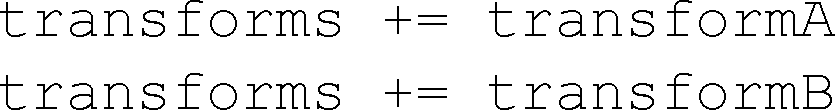
\includegraphics[width=0.7\textwidth]{figures/transform2.pdf}
  \label{fig:transform2}
  \end{subfigure}
\caption{Elaboration Time Interface}
\label{fig:transforms}
\end{figure}

\subsection{When}
Chisel provides a {\tt when - elsewhen - otherwise} statement for
performing conditional updates on {\tt Bits} and {\tt Reg}
nodes. This statement appears behaviorial but actually constructs a
hardware circuit to perform the update. The construction of this
circuit is delayed until elaboration time since it is easier to
construct the circuit once the user has specified all the updates than
it is to construct the circuit as the user is specifying
updates. 

{\bf Runtime}. Instead of constructing hardware whenever a {\tt when}
statement is executed, we simply record information to be used during
elaboration. For this purpose, we maintain a mapping of node to list
of update tuples with the format {\tt (cond, bits)} where {\tt cond}
is the condition of the when statement and {\tt bits} is the update
data. These update tuples are constructed for every update statement
within the body of a {\tt when} statement and appeneded to the list
mapped to the node on the left hand side of that update
statement. Note that the updates in this list do not have to be
mutually exclusive. In the case when multiple updates are enabled,
Chisel has the semantics that the last update in program order (i.e
the last update in the list of updates) takes priority.

{\bf Elaboration time}. The elaboration time transformation function
does not need to perform any analysis since all the elaboration
information is already logged.

\subsection{SRAM Interface}

\subsection{Automatic Pipeline Synthesis}
